\subsection{ArrowParallel Implementations}
\begin{frame}[fragile]{GpH}
\begin{lstlisting}[frame=htrbl]
data Conf a = Conf (Strategy a)

instance (ArrowChoice arr) =>
  ArrowParallel arr a b (Conf b) where
    parEvalN (Conf strat) fs =
        evalN fs >>>
        arr (withStrategy (parList strat))
\end{lstlisting}
\begin{center}
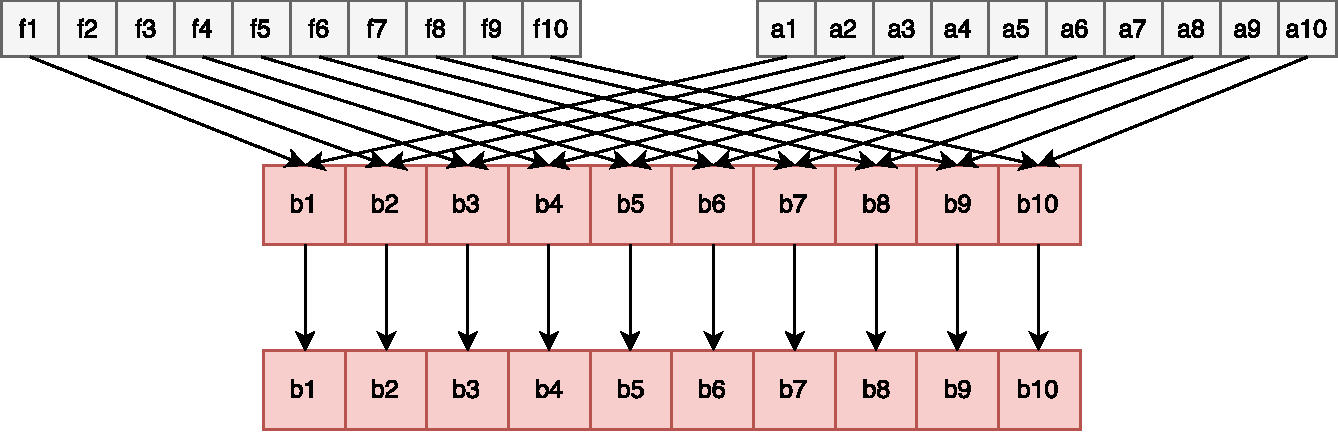
\includegraphics[scale=0.45]{images/parEvalNMulticore}
\end{center}
\end{frame}

\begin{frame}[fragile]{Par Monad}
\begin{lstlisting}[frame=htrbl]
type Strategy a = a -> Par (IVar a)
data Conf a = Conf (Strategy a)

instance (ArrowChoice arr) => ArrowParallel arr a b (Conf b) where
    parEvalN (Conf strat) fs =
        evalN (map (>>> arr strat) fs) >>>
        ...
\end{lstlisting}
\begin{center}
\includegraphics[scale=0.4]{images/parEvalNParMonad1}
\end{center}
\end{frame}

\begin{frame}[fragile]{ParMonad}
\begin{lstlisting}[frame=htrbl]
        ...
        arr sequenceA >>>
        arr (>>= mapM Control.Monad.Par.get) >>>
        arr runPar
\end{lstlisting}
\begin{center}
\includegraphics[scale=0.4]{images/parEvalNParMonad2}
\end{center}
\end{frame}


\begin{frame}[fragile]{Eden problems}
For Eden we need separate implementations.\\~\\
This is because of \code{spawnF} only supporting functions \lstinline{(->)}:
\begin{lstlisting}[frame=htrbl]
spawnF :: (Trans a, Trans b) => [a -> b] -> [a] -> [b]
\end{lstlisting}
\pause
Hacky alternative:
\begin{lstlisting}[frame=htrbl]
class (Arrow arr) => ArrowUnwrap arr where
    arr a b -> (a -> b)
\end{lstlisting}
\end{frame}

\begin{frame}[fragile]{Eden implementation - Functions}
Straightforward:
\begin{lstlisting}[frame=htrbl]
data Conf = Nil

instance (Trans a, Trans b) => ArrowParallel (->) a b conf where
	parEvalN _ = spawnF
\end{lstlisting}
\begin{center}
\includegraphics[scale=0.5]{images/parEvalNEden}
\end{center}
\end{frame}

\begin{frame}[fragile]{Eden implementation - Kleisli}
Implementation for the Kleisli Type:
\begin{lstlisting}[frame=htrbl]
instance (ArrowParallel (->) a (m b) Conf,
  Monad m, Trans a, Trans b, Trans (m b)) =>
  ArrowParallel (Kleisli m) a b conf where
    parEvalN conf fs = 
      arr (parEvalN conf (map (\(Kleisli f) -> f) fs)) >>>
      Kleisli sequence
\end{lstlisting}
\begin{center}
\includegraphics[scale=0.5]{images/parEvalNEden}
\end{center}
\end{frame}